\documentclass[dcc]{fcfmcourse}
\usepackage{teoria}
\usepackage[utf8x]{inputenc}
\usepackage{amsmath}
\usepackage{amsfonts,setspace}
\usepackage{listings}
\usepackage{color}

\definecolor{pblue}{rgb}{0.13,0.13,1}
\definecolor{pgreen}{rgb}{0,0.5,0}
\definecolor{porange}{rgb}{0.9,0.5,0}
\definecolor{pgrey}{rgb}{0.46,0.45,0.48}

\lstset{language=Java,
  showspaces=false,
  showtabs=false,
  breaklines=true,
  showstringspaces=false,
  breakatwhitespace=true,
  commentstyle=\color{porange},
  keywordstyle=\color{pblue},
  stringstyle=\color{pgreen},
  basicstyle=\ttfamily,
  moredelim=[il][\textcolor{pgrey}]{$ $},
  moredelim=[is][\textcolor{pgrey}]{\%\%}{\%\%}
}

\newenvironment{codebox} {\small \ttfamily \obeylines \begingroup \setstretch{-2.4}} {\endgroup}

% Sugerencias para un mejor titulo?
\title{Auxiliar 3 - Análisis matemático de algoritmos}
\course[CC3001]{Algoritmos y Estructuras de Datos}
\professor{Nelson Baloian}
\professor{Patricio Poblete}
\assistant{Manuel Cáceres}
\assistant{Sebastián Ferrada}
\assistant{Sergio Peñafiel}

% Si pasas el comando usedate a la clase, la fecha aparecerá bajo la lista de auxiliares.
% Puedes usar el formato de fecha por defecto de latex (y traducirla usando babel)
% o puedes escribir lo que quieras con el comando \date.
% \date{1 de Septiembre, 2015}


\begin{document}
\maketitle

\vspace{-1ex}

\begin{problems}
\problem \textbf{StoogeSort.}\\
StoogeSort es un algoritmo de ordenación de arreglos que se basa en el principio de dividir para reinar. Su funcionamiento para ordenar un arreglo A de tamaño n es el siguiente: 

\begin{itemize}
    \item Se analiza el primer y el último elemento del arreglo, si el primero es mayor se intercambia con el último.
    \item Se divide el arreglo A en 3 sub-arreglos de tamaño n/3
    \item Se aplica StoogeSort sobre los primeros 2n/3 elementos del arreglo.
    \item Se aplica StoogeSort sobre los últimos 2n/3 elementos.
    \item Se vuelve a aplicar StoogeSort sobre los primeros 2n/3 elementos del arreglo
\end{itemize}

A partir de lo anterior:

\begin{enumerate}
    \item Implemente la función \texttt{public static void StoogeSort(float[] A, int inicio, int fin)} que ordena según StoogeSort
    \item Analice la complejidad del algoritmo, discuta sobre este resultado comparándolo con \texttt{BubbleSort} y \texttt{QuickSort}.
\end{enumerate}

\problem \textbf{Similitud genética (Subsecuencia común más larga)}

El ADN puede ser representado como una secuencia de strings (A,C,G,T); las secuencias de distintas bases nitrogenadas(caracteres) definen genes en el ADN. En biología, un problema de gran interés es encontrar la similitud entre distintas hebras de ADN. Para esto debemos encontrar cuán parecido son 2 strings $X$ e $Y$. Una de medida de similitud consiste en encontrar la subsecuencia común más larga a ambas. \\

Siendo z, x 2 strings cualesquiera diremos que z es subsecuencia de x si podemos obtener z al extraer 0 o más caracteres de x. (Observe que no es lo mismo que ser substring). Por ejemplo, ''electra", ''once", ''grita" son subsecuencias de ''electroencefalografista".\\

Para encontrar esta subsecuencia más larga podemos revisar todas las subsecuencias de $X$ y comprobar si también es subsecuencia de $Y$ retornando la más larga que cumpla esta propiedad. Sin embargo, esta solución revisa cada una de las $2^{|X|}$ subsecuencias de $X$, por lo que el algoritmo es ineficiente.\\

Proponga soluciones más eficientes a esta, e implemente la mejor.\\
\textbf{Hint:} La solución del problema posee subestructuras óptimas (Programación Dinámica)


\problem \textbf{Maratón de películas! (Maximización de tareas)}\\
Alicia y Roberto quieren ver la mayor cantidad de películas este fin de semana. Para esto Roberto revisa la programación de $TODOS$ los canales de televisión obteniendo un conjunto de $n$ películas $\mathcal{P} =\lbrace [i_{0},f_{0}],\ \ldots \ , [i_{n-1},f_{n-1}] \rbrace$ (donde $i_{k}$ y $f_{k}$ corresponden a los tiempos de inicio y fin de la película $k$) y le pide a Alicia que escoja la mayor cantidad de películas de modo que puedan verlas todas de inicio a fin.\\

Alicia no sabe programar pero considera que el siguiente algoritmo(escrito en pseudocódigo) funcionaría:
\begin{center}
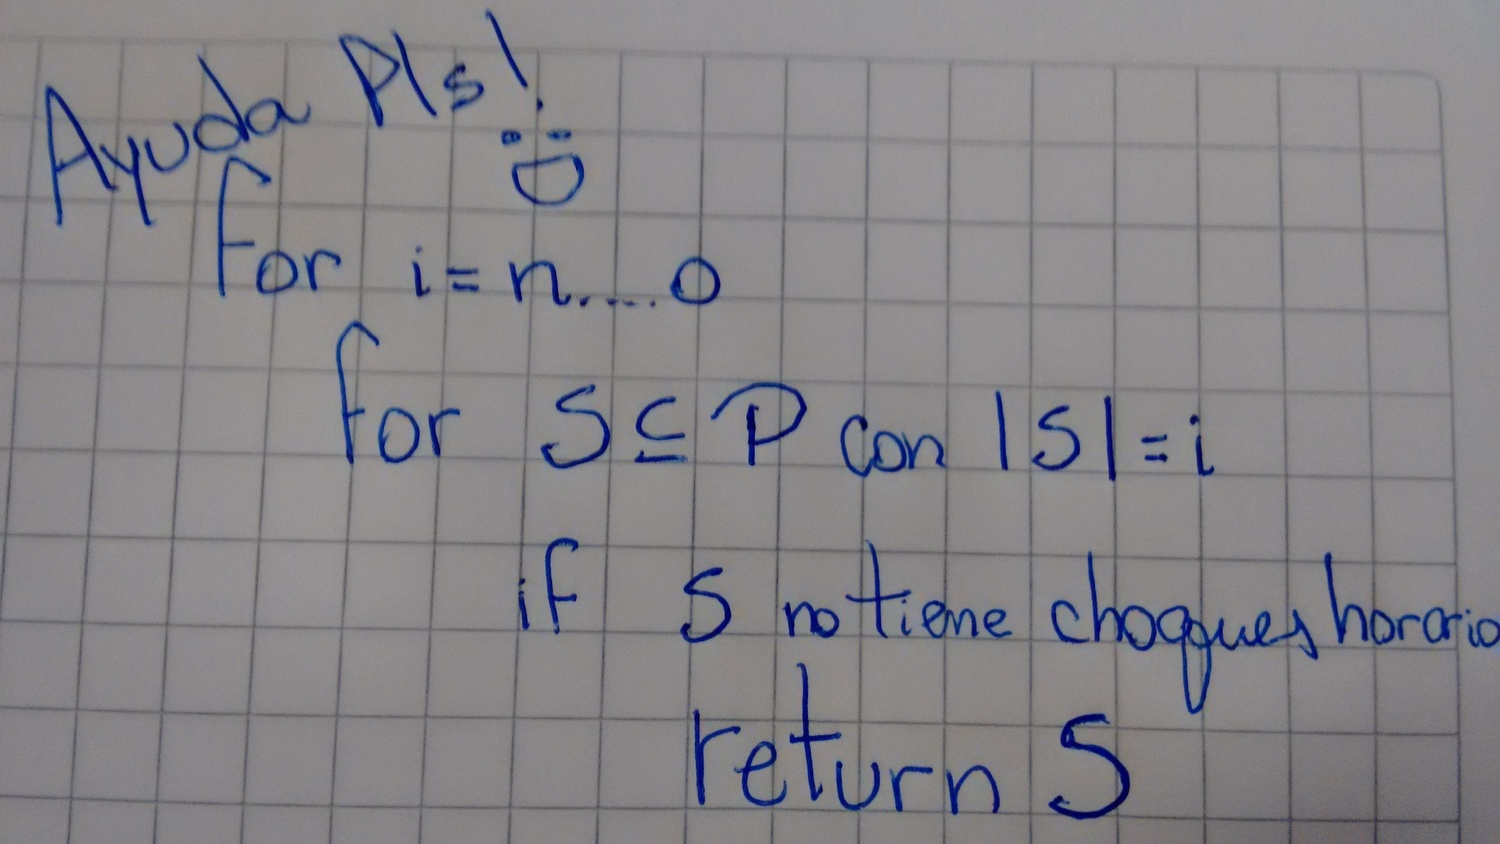
\includegraphics[scale=0.18]{Algoritmo.jpg}
\end{center}
Para lo que sigue considere que los tiempos de $P$ están en una matriz de $n \times 2$ y solo retorne la cantidad de películas escogidas.
\begin{enumerate}
    \item Implemente el pseudocódigo escrito por Alicia como una función\\ \texttt{public static int maximoPeliculas(int [][] P)}
    \item Considere que es Viernes (poco tiempo para el fin de semana) y que Roberto recolectó muchas películas ¿Qué problema tiene esta solución?
    \item Implemente nuevamente la función, pero más eficientemente.\\
    \textbf{Hint:} Sea avaro
    \item \textbf{Propuesto:} Modifique las funciones anteriores de modo que retornen un \texttt{int []} que tenga los índices en P de las películas escogidas.
\end{enumerate}
\end{problems}

\end{document}
